\chapter{The Algorithm}
\label{The Algorithm}

The problem of finding convincing parameters for the filters can be divided into several sub-problems. Figure ~\ref{fig:problem} shows the individual steps of the process.

\begin{figure}[htb]
  \centering  
  \caption{sub-problems of parameter extraction}
  \label{fig:problem}
	\begin{tikzpicture}[auto, thick, node distance=2.1cm, >=triangle 45]
	
		\draw node at (0,0) [block] (ir) {\Large$Impulse\ Resonse$};
		\draw node [block, below of=ir] (FFT) {\Large$Extraction\ of\ Resonance\ Signal\ Spectrum$};
		\draw node [block, below of=FFT] (choose) {\Large$Finding\ the\ Most\ important\ Frequencies$};
		\draw node [block, below of=choose] (pars) {\Large$Determining\ amplitude\ and\ decay$};
		
		
		\draw[->] (ir) -- node {}(FFT);
		\draw[->] (FFT) -- node {}(choose);
		\draw[->] (choose) -- node {}(pars);
		
	\end{tikzpicture}
\end{figure}

The problem of obtaining a proper impulse response is not discussed here, rather the emphasis lies on the automated or semi-automated processing of the data. Each of the blocks in figure ~\ref{fig:problem} is a complex process of its own. Therefore each of these will be treated individually here. \\

\section{Extraction of Resonance Spectral Data}
\label{subsec:extraction}



The extraction of spectral data from a given signal is typically done using the fast fourier transform. But since this document assumes that the excitation of the body happens in a suboptimal manner, it is reasonable to assume that techniques to distinguish between source and resonator apply. 
Such techniques are for example described in \citep[p. 87]{cook_real_2002}. Here, particularly linear prediction coding (LPC) and autocorrelation are emphasized as a method for on the one hand distinguishing between source and resonator or filter and residual and on the other hand synthesizing a simulation of exciting the resonator with an arbitrary excitation signal. Cook uses autocorrelation to derive coefficients of a linear prediction, which is equivalent to convolution with the coefficients interpreted as the convolution kernel. This document aims towards using IIR filters so the exact procedure does not apply. Nevertheless, assuming autocorrelation is outputting the spectrum of the impulse response of the resonator, it is useful for IIR coefficient approximation. It is a starting point for the next sub-problem of peak finding in that spectrum. \\
In figure ~\ref{fig:spectrumAnalyse} the general idea is presented. This data flow contains a lot of redundancy and is only meant to explain the way from sampled impulse response, \(h_1[n]\), to it's autocorrelation done in the frequency domain(by multiplication with the signal's complex conjugate), getting the impulse response of the resonator \(h_2[n]\), to finally arrive at the frequency response of the resonator \(H_2[k]\). Many optimizations can be introduced in the processing presented in fig. ~\ref{fig:spectrumAnalyse}. 

\begin{figure}[htb]
  \centering  
  \caption{Extraction of spectral data}
  \label{fig:spectrumAnalyse}
	\begin{tikzpicture}[auto, thick, node distance=2.1cm, >=triangle 45]
	
		\draw node at (0,0) [input] (ir1) {};

		\draw node [block, right of=ir1] (FFT) {\Large$FFT$};
		\draw node at (4,-2)[block] (conj) {$\overline{x}$};
		\draw node at (6,0)[mult] (conv) {};
		\draw node [block, right of=conv] (iFFT) {\Large$iFFT$};
		\draw node at (11,0)[block] (FFT2) {\Large$FFT$};

		\draw node [output, right of=FFT2] (out) {};
		

		\draw[->] (ir1) -- node {\Large$h_1[n]$}(FFT);
		\draw[->] (FFT) -- (3,0) |- node {}(conj);
		\draw[->] (3,0) -- node {$H_1[k]$}(conv);
		\draw[->] (conj.east) -|  node [right,pos=0.5] {$\overline{H_2[k]}$}(conv); 
		\draw[->] (conv) -- node {}(iFFT);
		\draw[->] (iFFT) -- node {$h_2[n]$}(FFT2);
		\draw[->] (FFT2) -- node {\Large$H_2[k]$}(out);
		\draw node at (3,0) {\textbullet};
	\end{tikzpicture}
\end{figure}

To prove and test the behavior of the general idea presented in fig. ~\ref{fig:spectrumAnalyse} the plot shown below, fig. ~\ref{fig:specVsCorr} has been produced. The signal being analyzed here is composed of white noise at 0 dB FS and a sine wave at -20dB FS with a frequency of 1 kHz. Clearly, both the spectrum and the autocorrelation show a peak at 1 kHz, but the spectrum is much noisier.

\begin{figure}[h]
	\begin{center}
		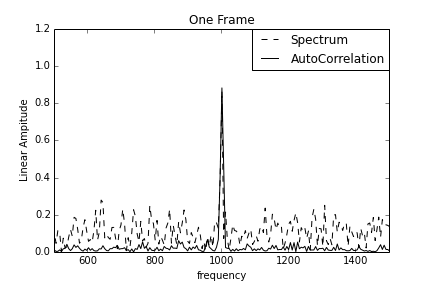
\includegraphics[width = 10cm]{img/specVsCorr.png}
		\caption{Spectrum and autocorrelation of a test signal}
		\label{fig:specVsCorr}
	\end{center}
\end{figure}

Since ultimately, the aim is to automatically find strong, persistent sinusoidal components in the impulse response, the behavior of autocorrelation seems ideal. Since the presented algorithm takes an impulse resonse and outputs an impulse response, it can easily be cascaded to even more attenuate noise and emphasize sinusoids. This can dramatically reduce the challenges for the peak finding algorithm that follows the spectrum extraction. Figure ~\ref{fig:multipassCorr} shows the noise reduction. Depending on the peak detection algorithm used and the signal to be analyzed, a second autocorrelation pass can both improve the signal to noise ratio but also reduce amplitude differences between sinusoidal components. Therefore, it can have a negative effect on an algorithm that tries to find out what components are more important(more loud in the simplest case) than other ones. All three frames have been individually normalized to show the peak at a linear amplitude of 1.    

\begin{figure}[h]
	\begin{center}
		\includegraphics[width = 10cm]{img/multipass.png}
		\caption{The spectrum vs. the autocorrelation, vs. a second autocorrelation pass (from top to bottom)}
		\label{fig:multipassCorr}
	\end{center}
\end{figure}

\section{Deciding which frequencies are important}
\label{subsec:peakDetection}
The decision which frequencies in a spectrum are the most important ones is crucial since it can reduce the number of resonant bandpass filters needed to produce a convincing result. The lower the number of frequencies, the more controllable, meaningful and efficient the solution will be. The final filter bank is supposed to run in real time to reinforce experimentation and easy manipulation of the model, which is one of it's advantages over the convolution approach. Here, a more complex signal is needed than the introduced simple test signal. A recording of a trash bucket, depicted below in figure ~\ref{trash} ,is used for this purpose.   


\begin{figure}[h]
	\begin{center}
		\includegraphics[width = 10cm]{img/trash.png}
		\caption{a metal trash bucket has been used to obtain a test impulse response}
		\label{trash}
	\end{center}
\end{figure}

The bucket has been hit using a standard drumstick to record the impulse response shown in fig ~\ref{kuebelIr}.

\begin{figure}[h]
	\begin{center}
		\includegraphics[width = 10cm]{img/kuebelIr.png}
		\caption{The impulse response recording of the bucket}
		\label{kuebelIr}
	\end{center}
\end{figure}

As described, the first step in finding the peaks is going to the frequency domain and applying autocorrelation. But even further, the spectrum of the autocorrelation can be accumulated over time. One frame of the spectrum of the impulse response and the accumulated spectrum of the autocorrelated signal are shown in fig. ~\ref{compare}. As shown later, the resulting application will allow a user to use either the spectrum, the autocorrelation, an accumulated autocorrelation or a two-pass autocorrelation as a basis for the analysis.



\begin{figure}[h]
	\begin{center}
		\includegraphics[width = 15cm]{img/compare.png}
		\caption{Comparison of a frame of the spectrum to the accumulated spectrum of the autocorrelated signal}
		\label{compare}
	\end{center}	
\end{figure}




% \begin{figure}[h]
	% \begin{center}
		% \includegraphics[width = 15cm]{img/compare.png}
		% \caption{Comparison of a frame of the spectrum to the accumulated spectrum of the autocorrelated signal}
		% \label{compare}
	% \end{center}
% \end{figure}

Accumulation has now been added to the process to further be sure that the strongest and most long lasting frequencies are present in the signal to be analyzed. A last step will be smoothing the spectral data using convolution, which will be described in ~\ref{subsec:preprocess}. Therefore the whole processing can be described as shown in fig. ~\ref{fig:Algorithm}. 

\begin{figure}[h!]%[htb]
  \centering  
  \caption{A high-level few of the algorithm}
  \label{fig:Algorithm}
	\begin{tikzpicture}[auto, thick, node distance=2.1cm, >=triangle 45]
	
		\draw node at (0,0) [block] (ir) {\Large$h[n]$};
		\draw node [block, below of=ir] (ac) {\Large$autocorrelation$};
		% \draw node [block, below of=ac] (FFT) {\Large$FFT$};
		\draw node [block, below of=ac] (accu) {\Large$accumulation\ filter$};
		\draw node [block, below of=accu] (filter) {\Large$Freq\ domain\ smoothing\ filter$};
		\draw node [block, below of=filter] (maxima) {\Large$Find\ Local\ Maxima$};
		
		\draw[->] (ir) -- node {}(ac);
		% \draw[->] (ac) -- node {}(FFT);
		\draw[->] (ac) -- node {$Magnitude\ Data$}(accu);
		\draw[->] (accu) -- node {}(filter);
		\draw[->] (filter) -- node {$smoothed\ Magnitude\ Data$}(maxima);
	\end{tikzpicture}
\end{figure}



Peak finding is a problem that has many solutions. ~\citep{scholkmann_efficient_2012} list a couple of known algorithms that are capable of finding local maxima or multiple peaks in given data. Here, a very primitive heuristic solution will be used: a python script that, with some modification, is able to run inside Max/MSP to iterate over given spectral data. 

\section{The Excitation Signal}
\label{subsec:exciter}
The simplest excitation signal is the unit sample, \(\delta[n]\). One could say, it is the simplest signal in general. In case of a convolution approach using just the IR as a coefficient set (or kernel), without the autocorrelation step, \(\delta[n]\) as an exciter would just reproduce the IR exactly. The autocorrelation step is, as mentioned, thought as a process of dividing resonator and exciter. Or to be more concrete, it's dividing periodic and non-periodic components. The output of the autocorrelation can be used to reveal the excitation signal. When the autocorrelation is done in the frequency domain it can simply be achieved by a single complex multiplication. This can be done as follows: multiplying the imaginary part of the FFT coefficients by -1 to get the complex conjugate of the signal. After that, convolution (a complex multiplication) of the original signal with its complex conjugate is performed. This provides the autocorrelation signal. The amplitude coefficients of the autocorrelation can now be subtracted from the amplitude coefficients or the original (clipping to 0) to synthesize the residual. The residual's spectrum as well as it's shape and duration can be very helpful in estimating what a good, natural sounding excitation signal could be for a given synthesis problem. For example if one would like to synthesize a sound similar to the provided IR, but just hit the body with a softer object, one could try to synthesize a signal similar to the residual. Or one could just use a low-pass filtered version of the residual right away.

    \begin{figure}[h]
    	\begin{center}
    		\includegraphics[width = 11cm]{img/AutoCorrAndResidual.png}
    		\caption{autocorrelation process, synthesizing an autocorrelated IR (to be analyzed in another patcher) and synthesizes a residual signal.}
    		\label{fig:acAndResidual}
    	\end{center}
    \end{figure}
In figure \ref{fig:residual} the smoothed spectrum of the calculated exciter of the trash bucket IR is shown in black. Obviously, it is quite flat. This seems to suggest a burst of noise, slightly low-pass filtered. The lower green graph is a synthesized approximation to the residual. White noise has been used, filtered with a simple one-pole at 1 kHz, to produce the approximation spectrum.


\begin{figure}[h]
	\begin{center}
		\includegraphics[width = 12cm]{residualTrashBucket2.png}
		\caption{Residual Signal spectrum of the trash bucket IR on top, black. A synthesized approximation below in green.}
		\label{fig:residual}
	\end{center}
\end{figure}






    
    









